%======================================================================
%  Anexo B - Modelo conceptual global
%======================================================================

\section{Modelo conceptual global}
\label{anx:global}

Este anexo conserva el diseño conceptual de toda la empresa, del que se
extrajo el módulo priorizado. Las figuras siguen la notación descrita
al inicio del capítulo 3.

\subsection{Vistas por usuario}

La vista U4 está completa dentro del módulo (figura~\ref{fig:vistaU4}
y, en notación de Chen, figura~\ref{fig:vistaU4chen});
las vistas U2 y U3 se muestran aquí completas, con las entidades de
otros módulos (documentos del vehículo y capacitaciones en U2; contrato
y factura en U3).

\textbf{U5 -- Flota y mantenimiento:} el vehículo, dónde está asignado,
sus documentos, sus mantenimientos y los despachos en que se usó.
\textbf{U6 -- Asesor comercial:} el cliente, sus sedes, el contrato y
las tarifas por zona y modalidad. \textbf{U7 -- Facturación y cartera:}
ve los envíos como envíos \textit{del cliente} (relación
\textit{envía}), junto con pagos y reclamaciones. \textbf{U8 -- Talento
humano:} el empleado, su centro y sus capacitaciones con el resultado;
la zona y la licencia aparecen como atributos del empleado.

{\singlespacing
\begin{figure}[!htb]
\centering
\adjustbox{max width=\linewidth, max totalheight=0.42\textheight}{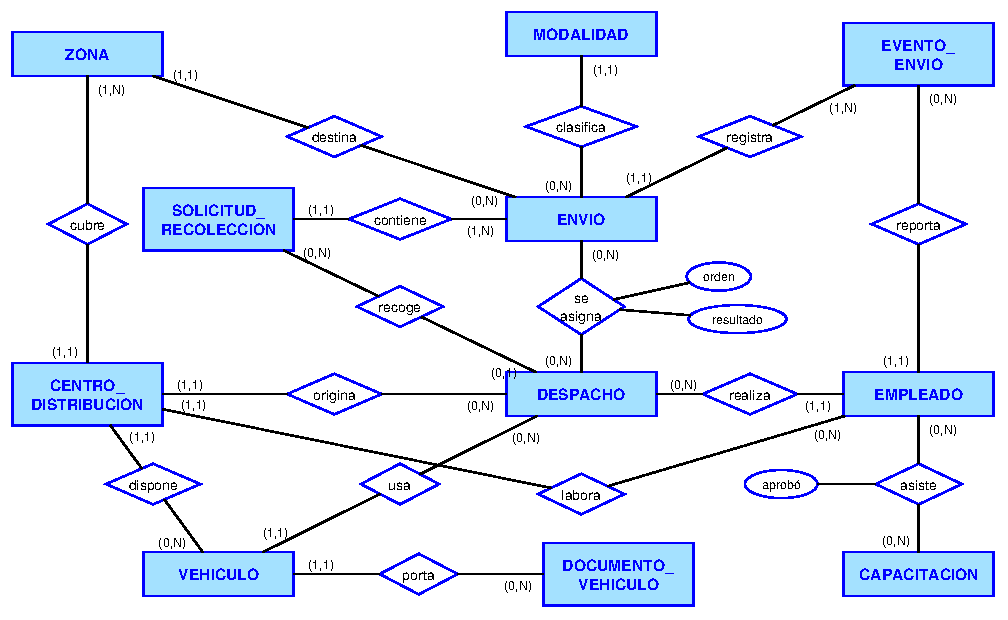
\includegraphics{figuras/er/U2.pdf}}
\caption{Vista U2 completa: personal del centro de distribución.}
\label{fig:vistaU2global}
\end{figure}
\par}
{\singlespacing
\begin{figure}[!htb]
\centering
\adjustbox{max width=\linewidth, max totalheight=0.42\textheight}{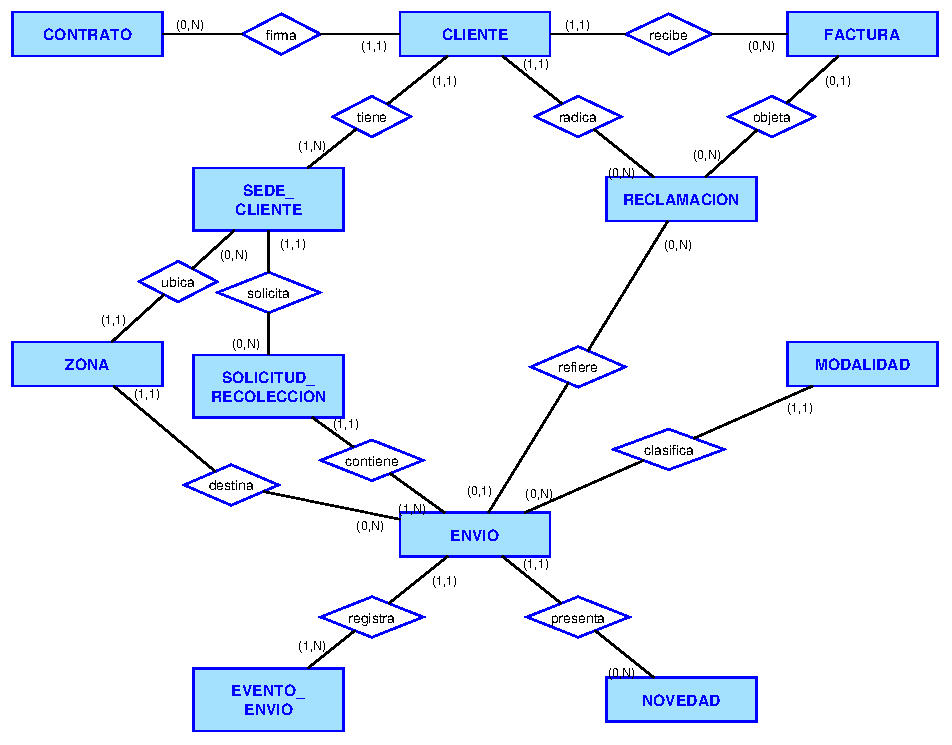
\includegraphics{figuras/er/U3.pdf}}
\caption{Vista U3 completa: mesa de servicio.}
\label{fig:vistaU3global}
\end{figure}
\par}
{\singlespacing
\begin{figure}[!htb]
\centering
\adjustbox{max width=\linewidth, max totalheight=0.3\textheight}{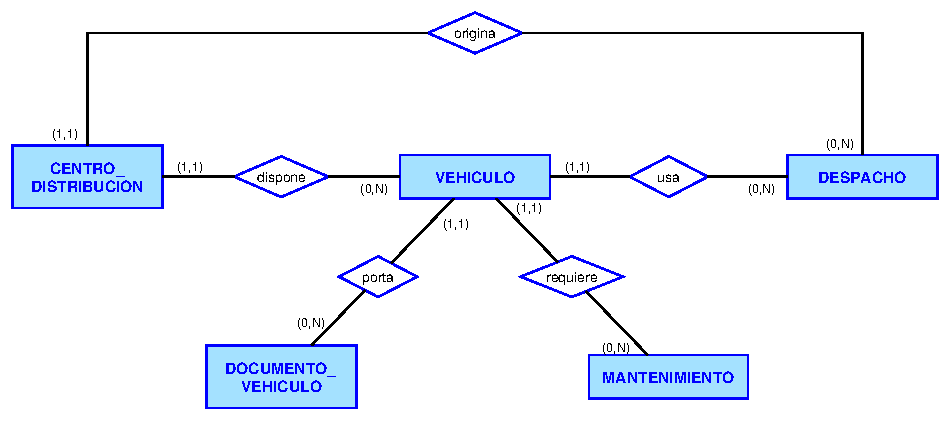
\includegraphics{figuras/er/U5.pdf}}
\caption{Vista U5: flota y mantenimiento.}
\label{fig:vistaU5}
\end{figure}
\par}
{\singlespacing
\begin{figure}[!htb]
\centering
\adjustbox{max width=\linewidth, max totalheight=0.3\textheight}{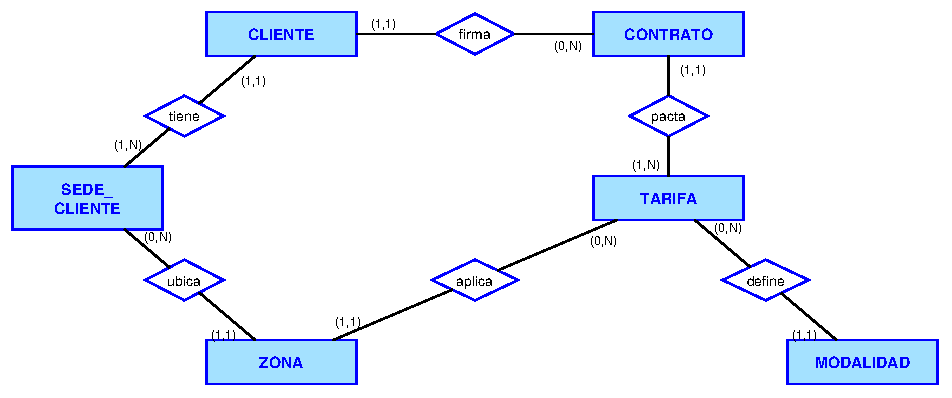
\includegraphics{figuras/er/U6.pdf}}
\caption{Vista U6: asesor comercial.}
\label{fig:vistaU6}
\end{figure}
\par}
{\singlespacing
\begin{figure}[!htb]
\centering
\adjustbox{max width=\linewidth, max totalheight=0.36\textheight}{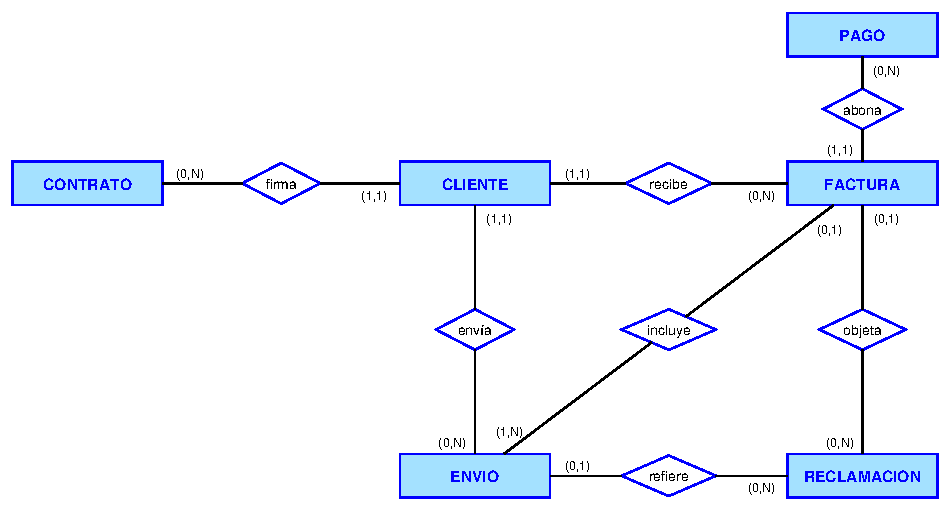
\includegraphics{figuras/er/U7.pdf}}
\caption{Vista U7: facturación y cartera.}
\label{fig:vistaU7}
\end{figure}
\par}
{\singlespacing
\begin{figure}[!htb]
\centering
\adjustbox{max width=\linewidth, max totalheight=0.2\textheight}{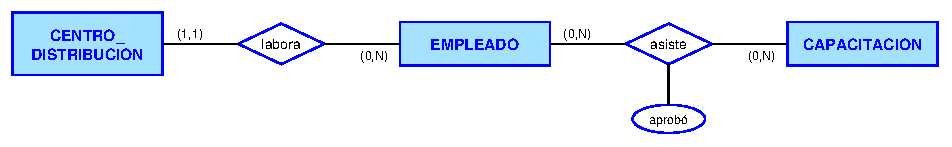
\includegraphics{figuras/er/U8.pdf}}
\caption{Vista U8: talento humano.}
\label{fig:vistaU8}
\end{figure}
\par}

\subsection{Prediseño global}

Integra las siete vistas con diagrama (U2 a U8): 21 entidades y 31
relaciones (figura~\ref{fig:erintegradoglobal} y
tabla~\ref{tab:relacionesglobal}). La relación directa
CLIENTE--\textit{envía}--ENVIO de la vista U7 se eliminó porque se
obtiene recorriendo CLIENTE--\allowbreak SEDE\_CLIENTE--\allowbreak SOLICITUD\_RECOLECCION--\allowbreak ENVIO;
guardar ambas permitiría asociar un envío a un cliente distinto del que
lo solicitó. Todas las demás vistas son subconjuntos del prediseño. La
zona fija del mensajero queda como atributo de EMPLEADO (defecto que
corrige el ajuste 3).

{\singlespacing\small
\begin{longtable}{L{1.5cm} L{5.0cm} L{2.2cm} L{5.4cm}}
\caption{Relaciones del prediseño global.}
\label{tab:relacionesglobal}\\
\toprule
\textbf{Relación} & \textbf{Entidades} & \textbf{(mín,máx)} & \textbf{Significado} \\
\midrule
\endfirsthead
\toprule
\textbf{Relación} & \textbf{Entidades} & \textbf{(mín,máx)} & \textbf{Significado} \\
\midrule
\endhead
\bottomrule
\endfoot
\textit{cubre} & CENTRO\_DISTRIBUCION --\allowbreak\ ZONA & (1,1) -- (1,N) & Cada zona es atendida por un solo centro. \\
\textit{labora} & CENTRO\_DISTRIBUCION --\allowbreak\ EMPLEADO & (1,1) -- (0,N) & Cada empleado trabaja en un centro. \\
\textit{dispone} & CENTRO\_DISTRIBUCION --\allowbreak\ VEHICULO & (1,1) -- (0,N) & Cada vehículo está asignado a un centro. \\
\textit{origina} & CENTRO\_DISTRIBUCION --\allowbreak\ DESPACHO & (1,1) -- (0,N) & Cada despacho sale de un centro. \\
\textit{ubica} & ZONA --\allowbreak\ SEDE\_CLIENTE & (1,1) -- (0,N) & Cada sede del cliente está en una zona. \\
\textit{destina} & ZONA --\allowbreak\ ENVIO & (1,1) -- (0,N) & Zona a la que va cada envío. \\
\textit{aplica} & ZONA --\allowbreak\ TARIFA & (1,1) -- (0,N) & Zona a la que corresponde cada tarifa. \\
\textit{tiene} & CLIENTE --\allowbreak\ SEDE\_CLIENTE & (1,1) -- (1,N) & Sedes de recolección de cada cliente. \\
\textit{firma} & CLIENTE --\allowbreak\ CONTRATO & (1,1) -- (0,N) & Contratos que ha tenido cada cliente. \\
\textit{pacta} & CONTRATO --\allowbreak\ TARIFA & (1,1) -- (1,N) & Tarifas acordadas en cada contrato. \\
\textit{define} & MODALIDAD --\allowbreak\ TARIFA & (1,1) -- (0,N) & Modalidad a la que corresponde cada tarifa. \\
\textit{clasifica} & MODALIDAD --\allowbreak\ ENVIO & (1,1) -- (0,N) & Modalidad contratada para cada envío. \\
\textit{solicita} & SEDE\_CLIENTE --\allowbreak\ SOLICITUD\_RECOLECCION & (1,1) -- (0,N) & Solicitudes hechas desde cada sede. \\
\textit{contiene} & SOLICITUD\_RECOLECCION --\allowbreak\ ENVIO & (1,1) -- (1,N) & Envíos que se recogen en cada solicitud. \\
\textit{recoge} & DESPACHO --\allowbreak\ SOLICITUD\_RECOLECCION & (0,1) -- (0,N) & Despacho de recolección que atiende cada solicitud. \\
\textit{se asigna} & ENVIO --\allowbreak\ DESPACHO & (0,N) -- (0,N) & Un envío puede salir en varios despachos (reintentos) y un despacho lleva muchos envíos. Atributos: orden, resultado. \\
\textit{registra} & ENVIO --\allowbreak\ EVENTO\_ENVIO & (1,1) -- (1,N) & Historial de estados de cada envío. \\
\textit{reporta} & EMPLEADO --\allowbreak\ EVENTO\_ENVIO & (1,1) -- (0,N) & Empleado responsable de cada evento. \\
\textit{soporta} & ENVIO --\allowbreak\ PRUEBA\_ENTREGA & (1,1) -- (0,1) & Constancia de recibo de cada envío. \\
\textit{presenta} & ENVIO --\allowbreak\ NOVEDAD & (1,1) -- (0,N) & Novedades ocurridas con cada envío. \\
\textit{radica} & CLIENTE --\allowbreak\ RECLAMACION & (1,1) -- (0,N) & Reclamaciones hechas por cada cliente. \\
\textit{refiere} & ENVIO --\allowbreak\ RECLAMACION & (0,1) -- (0,N) & Envío sobre el que trata una reclamación (opcional). \\
\textit{objeta} & FACTURA --\allowbreak\ RECLAMACION & (0,1) -- (0,N) & Factura sobre la que trata una reclamación (opcional). \\
\textit{recibe} & CLIENTE --\allowbreak\ FACTURA & (1,1) -- (0,N) & Facturas emitidas a cada cliente. \\
\textit{incluye} & FACTURA --\allowbreak\ ENVIO & (0,1) -- (1,N) & Factura en la que se cobra cada envío. \\
\textit{abona} & FACTURA --\allowbreak\ PAGO & (1,1) -- (0,N) & Pagos aplicados a cada factura. \\
\textit{porta} & VEHICULO --\allowbreak\ DOCUMENTO\_VEHICULO & (1,1) -- (0,N) & Documentos de cada vehículo. \\
\textit{requiere} & VEHICULO --\allowbreak\ MANTENIMIENTO & (1,1) -- (0,N) & Mantenimientos de cada vehículo. \\
\textit{usa} & VEHICULO --\allowbreak\ DESPACHO & (1,1) -- (0,N) & Vehículo con el que se hace cada despacho. \\
\textit{realiza} & EMPLEADO --\allowbreak\ DESPACHO & (1,1) -- (0,N) & Empleado (mensajero) que hace cada despacho. \\
\textit{asiste} & EMPLEADO --\allowbreak\ CAPACITACION & (0,N) -- (0,N) & Capacitaciones de cada empleado. Atributo: aprobó. \\
\end{longtable}
\par}

\begin{landscape}
{\singlespacing
\begin{figure}[p]
\centering
\adjustbox{max width=22.5cm, max totalheight=14.6cm}{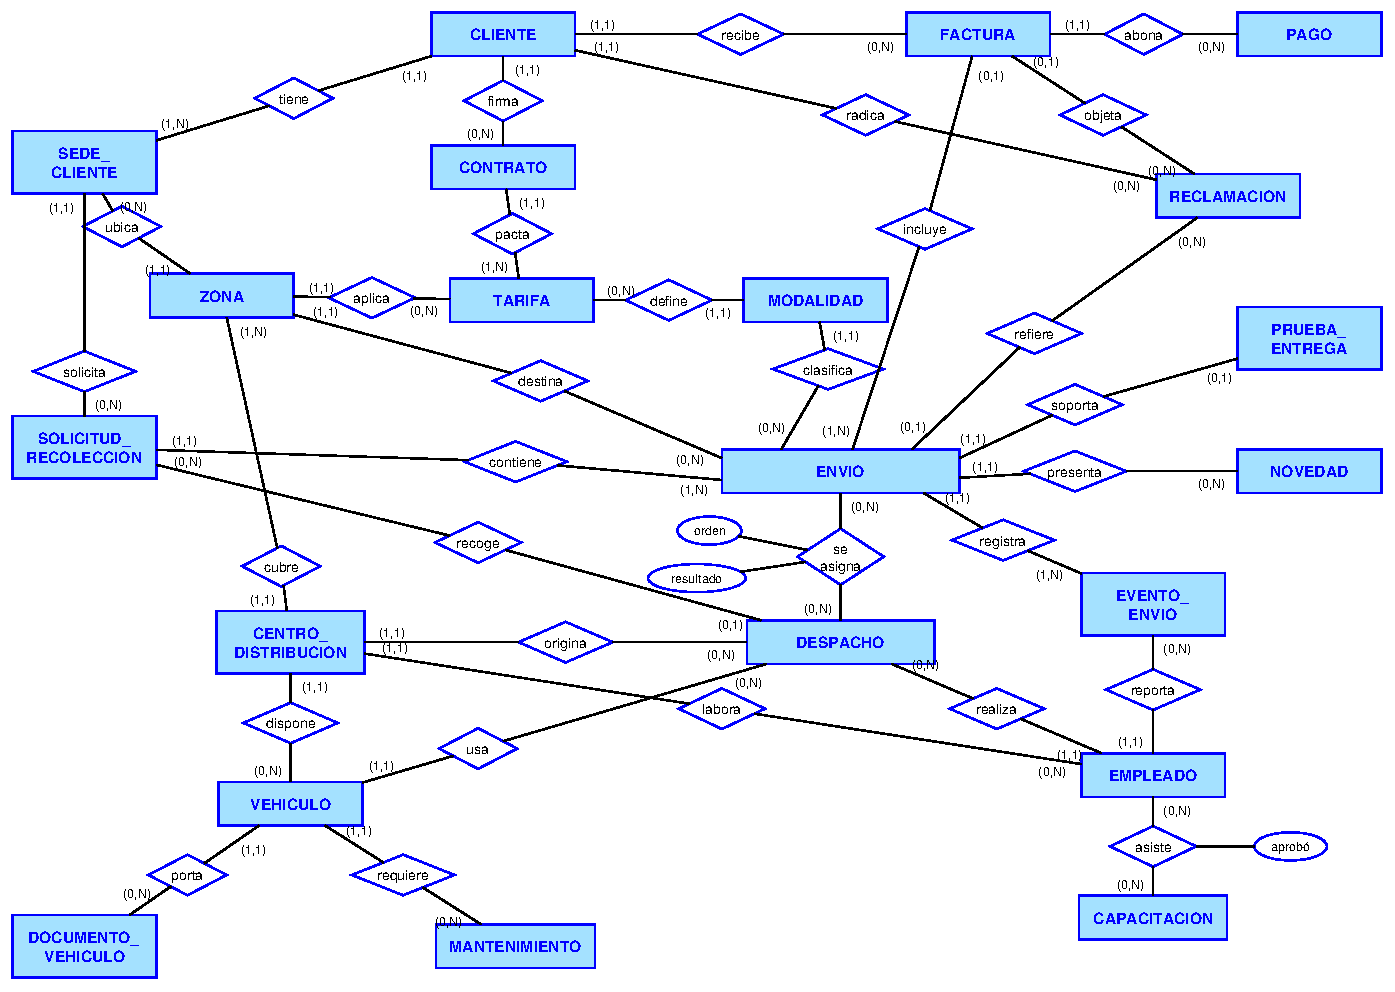
\includegraphics{figuras/er/prediseno.pdf}}
\caption{Prediseño conceptual global de BD\_ENLACE\_EXPRESS.}
\label{fig:erintegradoglobal}
\end{figure}
\par}
\end{landscape}


\subsection{Modelo ajustado global}

Con los ajustes 1 a 5 de la tabla~\ref{tab:ajustes}, el modelo global
pasa de 21 a 28 entidades. Se presenta en dos figuras según los grupos
de afinidad: la parte comercial y de operación (grupos G2, G3 y G4) y la
de recursos (G1, G5 y G6). Las entidades con fondo gris y borde punteado
aparecen en las dos figuras y se detallan en la otra. La
tabla~\ref{tab:atributosajustados} lista las entidades nuevas o
modificadas.

\begin{landscape}
{\singlespacing
\begin{figure}[p]
\centering
\adjustbox{max width=22.5cm, max totalheight=14.6cm}{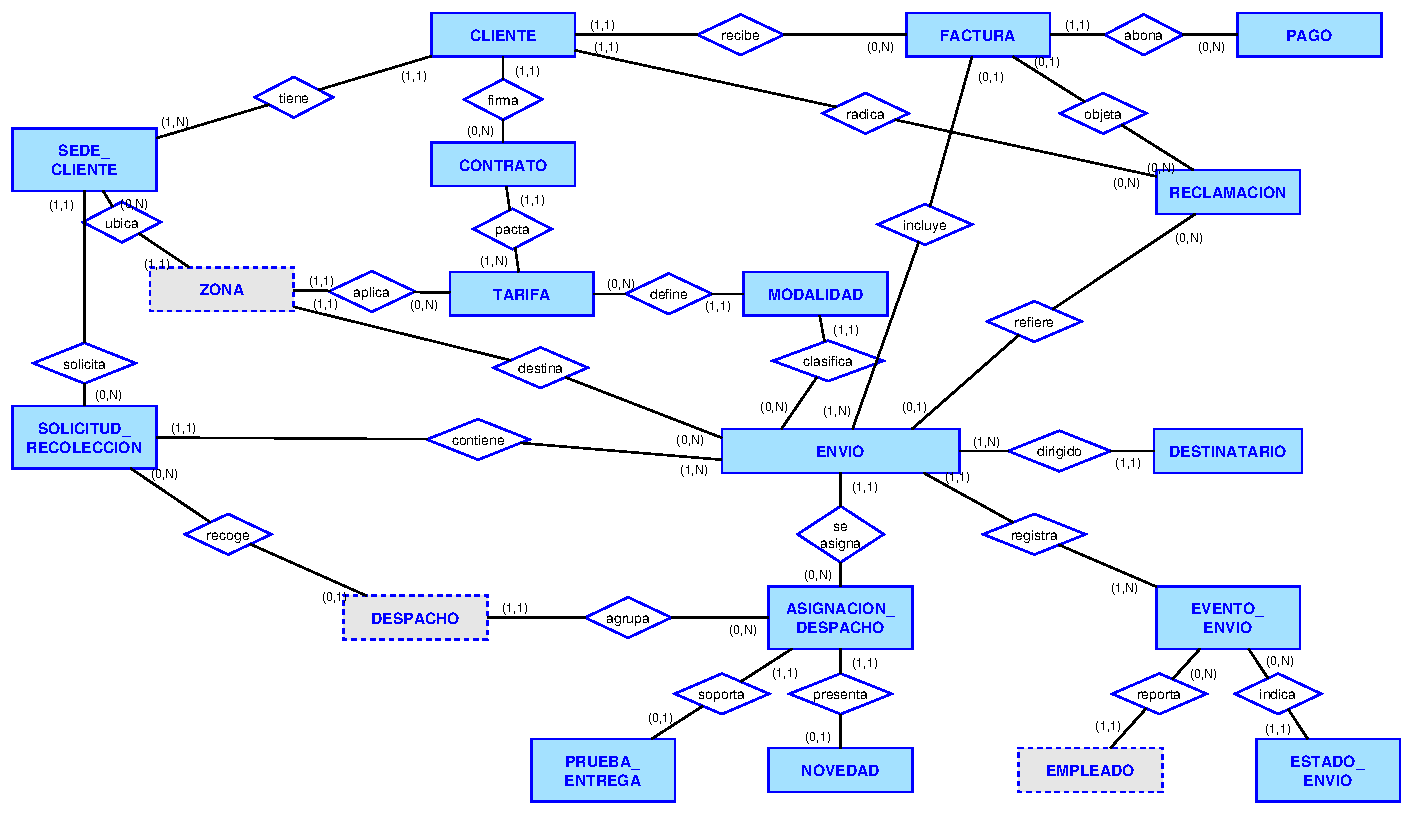
\includegraphics{figuras/er/ajustadoA.pdf}}
\caption{Modelo ajustado global: parte comercial y de operación de envíos.}
\label{fig:erfinalA}
\end{figure}
\par}
\end{landscape}
\begin{landscape}
{\singlespacing
\begin{figure}[p]
\centering
\adjustbox{max width=22.5cm, max totalheight=14.6cm}{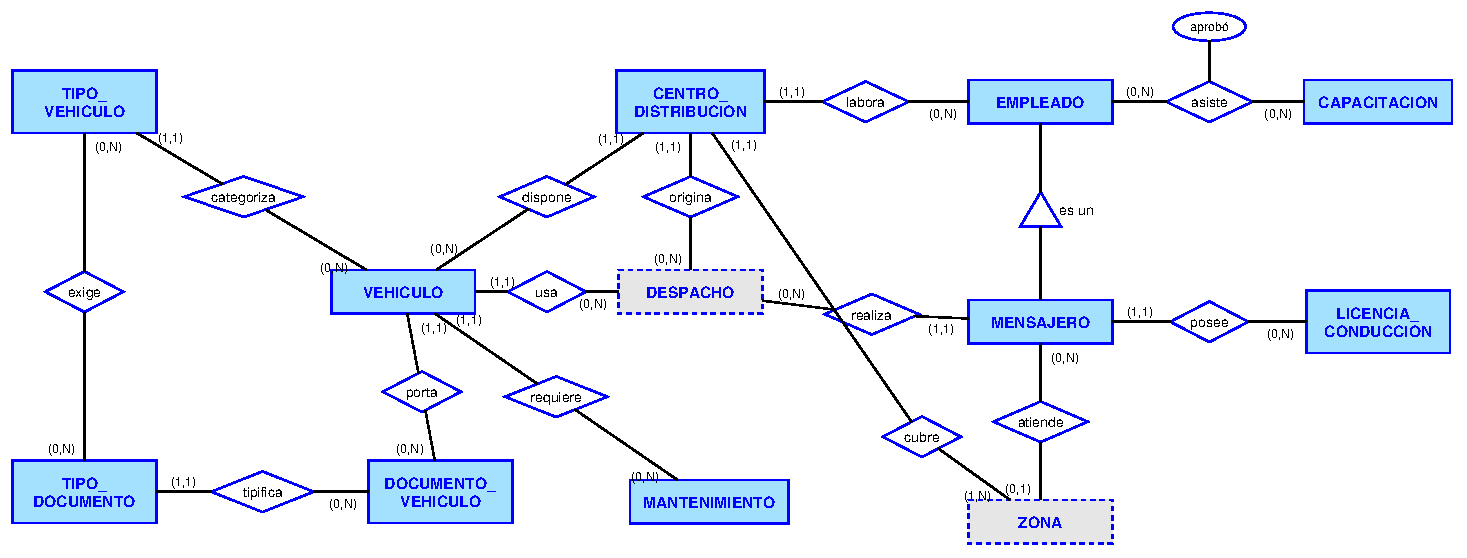
\includegraphics{figuras/er/ajustadoB.pdf}}
\caption{Modelo ajustado global: parte de recursos (centros, flota y personal).}
\label{fig:erfinalB}
\end{figure}
\par}
\end{landscape}
{\singlespacing\small
\begin{longtable}{L{3.6cm} L{3.4cm} L{7.4cm}}
\caption{Entidades nuevas o modificadas por los ajustes.}
\label{tab:atributosajustados}\\
\toprule
\textbf{Entidad} & \textbf{Estado} & \textbf{Atributos} \\
\midrule
\endfirsthead
\toprule
\textbf{Entidad} & \textbf{Estado} & \textbf{Atributos} \\
\midrule
\endhead
\bottomrule
\endfoot
DESTINATARIO & Nueva (ajuste 1) & id\_destinatario, tipo y número de documento, nombre, teléfono, correo \\
ENVIO & Modificada (ajustes 1 y 4) & número de guía, fecha de registro, dirección de destino, peso declarado, peso real, contenido, valor declarado, frágil, alto valor, valor del flete, fecha de compromiso \\
ASIGNACION\_\allowbreak DESPACHO & Nueva (ajuste 2) & id\_asignación, número de intento, orden de visita, hora de visita, resultado (pendiente, entregado, novedad, devuelto) \\
PRUEBA\_\allowbreak ENTREGA & Modificada (ajuste 2) & id\_prueba, fecha y hora, nombre y documento de quien recibe, tipo de prueba, archivo de soporte \\
NOVEDAD & Modificada (ajuste 2) & id\_novedad, tipo de novedad, descripción, acción (reintento o devolución), solución, estado \\
EMPLEADO & Modificada (ajuste 3) & id\_empleado, documento, nombres, apellidos, cargo, teléfono, correo, fecha de ingreso, fecha de retiro, motivo de retiro, estado \\
MENSAJERO & Nueva (ajuste 3) & id\_empleado (el mismo del empleado), tipo de vehículo que puede conducir \\
LICENCIA\_\allowbreak CONDUCCION & Nueva (ajuste 3) & id\_licencia, número, categoría, fecha de expedición, fecha de vencimiento \\
ESTADO\_ENVIO & Nueva (ajuste 4) & id\_estado, nombre (Registrado, Recolectado, En centro, Clasificado, En ruta, Entregado, Con novedad, Devuelto, Anulado), es final \\
EVENTO\_ENVIO & Modificada (ajuste 4) & id\_evento, fecha y hora, observación \\
TIPO\_VEHICULO & Nueva (ajuste 5) & id\_tipo\_vehículo, nombre (motocicleta, furgoneta, bicicleta eléctrica), capacidad máxima en kg \\
TIPO\_\allowbreak DOCUMENTO & Nueva (ajuste 5) & id\_tipo\_documento, nombre (SOAT, revisión técnico-mecánica, póliza, tarjeta de propiedad) \\
VEHICULO & Modificada (ajuste 5) & id\_vehículo, placa, marca, modelo, capacidad en kg, eléctrico, estado \\
DOCUMENTO\_\allowbreak VEHICULO & Modificada (ajuste 5) & id\_documento, número, fecha de expedición, fecha de vencimiento \\
\end{longtable}
\par}


